\begin{center}
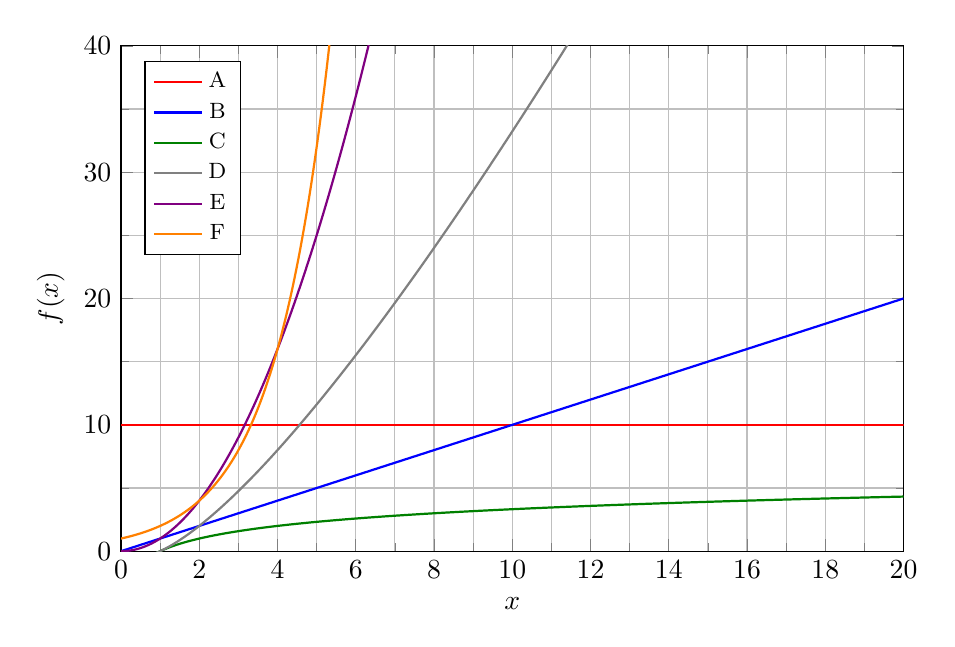
\begin{tikzpicture}
\begin{axis}[width=0.95\linewidth,height=8cm,xmin=0,xmax=20,ymin=0,ymax=40,xlabel={$x$},ylabel={$f(x)$},grid=both,minor tick num=1,
 every axis plot/.append style={thick},domain=0.01:20,samples=200,legend pos=north west,legend style={font=\footnotesize}]
\addplot[color=red] {10};
\addplot[color=blue] {x};
\addplot[color=green!50!black] {ln(x)/ln(2)};
\addplot[color=gray] {x*ln(x)/ln(2)};
\addplot[color=violet,domain=0:7] {x^2};
\addplot[color=orange,domain=0:6] {2^x};
\legend{A,B,C,D,E,F}
\end{axis}
\end{tikzpicture}
\end{center}
